\documentclass[12pt]{article}
\usepackage{fullpage,enumitem,amsmath,amssymb,graphicx}
\usepackage{listings}
\usepackage{tikz}
\usepackage{hyperref}
\usepackage{bbm}

\begin{document}

\begin{center}
{\Large CS 228 Winter 2018 Homework 5}

\begin{tabular}{rl}
SUNet ID: & 05794739 \\
Name: & Luis Perez \\
Collaborators: & \\
Late Days: & 0
\end{tabular}
\end{center}

By turning in this assignment, I agree by the Stanford honor code and declare
that all of this is my own work.

\section*{Problem 1}

\begin{enumerate}[label=(\alph*)]
  \item We wish to compute the Bayesian predictive probability of the described process using a Dirichlet prior. This is relatively straight-forward.

  \begin{align*}
  	P(X[M+1] = x^i \mid \mathcal{D}) &= \int_\theta P(X[M+1] = x^i, \theta \mid \mathcal D)d\theta \tag{integrate over all possible values of $\theta$} \\
  	&= \int_\theta P(X[M+1] = x^i \mid \theta, \mathcal{D})P(\theta \mid \mathcal{D}) d\theta \tag{Chain Rule} \\
  	&= \int_\theta P(X[M+1] = x^i \mid \theta)P(\theta \mid \mathcal{D}) \tag{$X \perp \mathcal{D} \mid \theta$} \\
  	&= \int_\theta \theta_i P(\theta \mid \mathcal{D}) \tag{definition of $P(X=x^k \mid \theta)$}\\
  	&= E_{\theta \sim P(\theta \mid \mathcal{D})}[\theta_i] 
  \end{align*}
  Therefore the problem simply boils down to figure out what form $P(\theta \mid D)$ takes. We note that:
  $$
  	P(\theta \mid D) \propto P(D \mid \theta) P(\theta)
  $$
  where $P(\theta)$ is a Dirichlet prior (ie, $P(\theta) \propto \prod_k \theta_k^{\alpha_k - 1}$) where $\theta \sim Dirichlet(\alpha_1, \cdots, \alpha_K)$. As per the hint, this implies that the posterior distribution $P(\theta \mid \mathcal{D})$ is given by $Dirichlet(\alpha'_1,\cdots,\alpha_K')$ where:
  $$
  	\alpha_k' = \alpha_k + \sum_{x[m] \in \mathcal{D}} \mathbbm{1}[x[m] = x^k]
  $$
  We therefore have the well-known result:
  \begin{align*}
  	E_{\theta \sim Dirichlet(\alpha_1', \cdots \alpha'_K)}[\theta_i] &= \frac{\alpha'_i}{\sum_k \alpha'_k} \\
  	&= \frac{\alpha_i + \sum_{j=1}^M \mathbbm{1}[x[j] = x^i]}{\sum_k \alpha_k + \sum_k \sum_{j=1}^M \mathbbm{1}[x[j] = x^k]} \\
  	&= \frac{\alpha_i + M[i]}{\alpha + M} \tag{the bottom just counts the total data samples and the top counts the samples matching $x^i$}
  \end{align*}
  The above is exactly what we desired.
  \item We now show how to compute the Bayesia predictive probability for two samples.
  \begin{align*}
  	P(X[M + 2] = x^j, X[M+1] = x^i \mid \mathcal{D}) &= P(X[M+2] \mid D \cup \{X[M+1] = x^i \})P(X[M+1] = x^i \mid \mathcal{D}) \tag{Chain rule where we consider $X[M+1]$ to just be another sample in our dataset} \\
  	&= \left(\frac{M[j] + \alpha_j}{M + 1+ \alpha}\right)\left(\frac{M[i] + \alpha_i}{M + \alpha}\right) \tag{In the case where $i \neq j$} \\
  	&= \left(\frac{M[i] + 1 + \alpha_i}{M + 1+ \alpha}\right)\left(\frac{M[i] + \alpha_i}{M + \alpha}\right) \tag{In the case where $i = j$}
  \end{align*}
  The above can be some simple because the posterior of the Dirichlet with a categorical likelihood is another Dirichlet, so we treat drawing the second sample simply as if we had had the first sample as part of our original dataset. Then the results follow directly from the result in part (a).

  \item Suppose that instead of computing the above we wish to use the approximation where we ignore the dependence between $X[M+1]$ and $X[M+2]$. Then we have:
  \begin{align*}
  	P(X[M+2] = x^j, X[M+1] = x^i \mid \mathcal{D}) &\approx P([X+1] = x^i \mid \mathcal{D})P(X[M+2] = x^j \mid \mathcal{D}) \\
  	&= \left(\frac{\alpha_i + M[i]}{M + \alpha}\right)\left(\frac{\alpha_j + M[j]}{M + \alpha}\right) \tag{results from (a)}
  \end{align*}
  We now consider the ratio of the approximation to the true probability. For $i = j$ we have:
  \begin{align*}
  	\frac{\frac{\alpha_i + M[i]}{M + \alpha}}{\frac{1 + \alpha_i + M[i]}{1 + \alpha + M}} \leq 1 \tag{since $\alpha_i + M[i] \leq \alpha + M$}
  \end{align*}
  We can consider two cases. Note that as $M \to \infty$, the ratio is:
  \begin{align*}
  	\lim_{M \to \infty} \frac{\frac{\alpha_i + M[i]}{M + \alpha}}{\frac{1 + \alpha_i + M[i]}{1 + \alpha + M}} &= \frac{\frac{\alpha_i + M[i]}{M}}{\frac{1 + \alpha_i + M[i]}{M}} \\
  	&= \frac{\alpha_i + M[i]}{1 + \alpha_i + M[i]} \\
  	&= 1 \tag{if we further assume that $x^i$ is generated with a non-zero probability}
  \end{align*}
  For small $M$ (ie, let's consider $M = 0$), we have:
  \begin{align*}
  \frac{\frac{\alpha_i}{\alpha}}{\frac{1 + \alpha}{1 + \alpha_i}} \leq 1 \tag{since $\alpha_i \leq \alpha$}
  \end{align*}
  Next, we consider the case where $i \neq j$. In this scenario, we have the ratio as:
  \begin{align*}
  	\frac{1 + \alpha + M}{\alpha + M} = 1 + \frac{1}{\alpha + M} > 1
  \end{align*}
  We can consider two cases. Note that as $M \to \infty$, the ratio is:
  \begin{align*}
  	\lim_{M \to \infty} 1 + \frac{1}{\alpha + M} &= 1
  \end{align*}
  For small $M$ (ie, let's consider $M = 0$), we have:
  \begin{align*}
  1 + \frac{1}{\alpha} > 1
  \end{align*}
  Therefore, from the above we can draw the following conclusions:
  \begin{itemize}
  	\item The more data we have, the closer the approximation is to the correct result. Intuitively, this makes sense, since the more samples we've collected, the more certain we are of our parameters $\theta$, and the less these are influenced by additonal samples. Therefore it becomes the case that the drawn samples will be independent.
  	\item The fewer the samples, the more strongly our prior affects our approximation. If we have very strong priors (large $\alpha_k$), then the closer our approximation is to the reality. If we have very weak priors and very few samples, then our approximation will be further from the true result.
  	\item In the case where we have few samples and weak priors, we note that our approximation is an under-estimate when $i = j$, and an over-estimates when $i \neq j$. Intuitively, this makes sense. If we have very weak priors and very little data and we sample $x^i$, then Bayesian, then we will believe that $x^i$ is very likely and will therefore assign high probability to sampling it again (compare this to our approximation, which ignores the fact we saw $x^i$ and will therefore under-estimate the probability of $x^i$ being sampled again). By a similar argument, with weak priors and few samples, if we see $x^i$, Bayesian theory will have use decrease the probabilities of seeing other values $x^j$ for $j \neq i$. However, our approximation will ignore this and will therefore over-estimate.
  \end{itemize}

\end{enumerate}

\section*{Problem 2}

\begin{enumerate}[label=(\Alph*)]
  \item Gaussian Mixture model
  	\begin{enumerate}[label=(\roman*)]
  		\item We can estimate the parameters for our mixture model relatively straight-forward, given the hidden variables $z_ij$. In fact, note that we have the log likelihood over our samples as (WLOG, we number the $5$ known precints as $i=1,\cdots,5$ and we set $\theta = (\pi, mu_0, mu_1, \Sigma_0, \Sigma_1)$.
  		\begin{align*}
  			\mathcal{L}(\mathcal{D}, \theta) &= \log P(\mathcal{D} \mid \theta) \\
  			&=\sum_{i=1}^N \sum_{j=1}^M \log P(X_{ij} = x_{ij}, Z_{ij} = z_{ij}) \\
  			&=\sum_{i=1}^N \sum_{j=1}^M \log \left[ (1-\pi)^{1-z_{ij}}\pi^{z_{ij}}\mathcal{N}(x_{ij} \mid \mu_{z_{ij}, \Sigma_{z_{ij}}})\right]
  		\end{align*}
  		Note that tbe above is not hard to optimzie, since we know the values $z_{ij}$ which tells us exactly which distribution each of the $X_{ij}$ belongs to. In fact, it is a well-known fact (as discussed in lecture) that the optimal parameters are:
  		\begin{align*}
  			\pi &= \frac{1}{NM} \sum_{i=1}^N \sum_{j=1}^M z_{ij} \\
  			\mu_0 &= \frac{\sum_{i=1}^N \sum_{j=1}^M (1 - z_{ij})x_{ij}}{\sum_{i=1}^N \sum_{j=1}^M (1-z_{ij})} \\
  			\mu_1 &= \frac{\sum_{i=1}^N \sum_{j=1}^M z_{ij} x_{ij}}{\sum_{i=1}^N \sum_{j=1}^M z_{ij}} \\
  			\Sigma_0 &= \frac{\sum_{i=1}^N \sum_{j=1}^M (1-z_{ij}) (x_{ij} - \mu_0)(x_{ij} - \mu_0)^T}{\sum_{i=1}^N \sum_{j=1}^M (1-z_{ij})} \\
  			\Sigma_1 &= \frac{\sum_{i=1}^N \sum_{j=1}^M z_{ij} (x_{ij} - \mu_1)(x_{ij} - \mu_1)^T}{\sum_{i=1}^N \sum_{j=1}^M z_{ij}}
  		\end{align*}
  		Using the labeled data, we arrive at the following estimates:
  		\begin{align*}
  		\pi &: 0.57 \\
			\mu_0 &: [[-0.99437209, -1.11730233]] \\
			\mu_1 &: [[1.04922807, 0.98085965]] \\
			\Sigma_0 &: [[0.30811884, 0.28553768], [0.28553768, 0.81346635]]\\
			\Sigma_1 &: [[0.77827888,0.19683566],[0.19683566, 0.24996938]]
		 \end{align*}
		\item We perform EM on the full data. We use three initializations - the first uses initializations from the parameters calculated in the previous section, and the second uses random initializations. See Figure \ref{fig:2aii} for a plot of the log likelihood over iteration for each initialization.

		The final parameters are:
		\begin{verbatim}
				{
				 'mu_0': matrix([[-1.04960572, -1.02771395]]),
				 'mu_1': matrix([[0.98435439, 0.99093038]]),
				 'sigma_0': matrix(
				 		[[0.35521351, 0.30612163],
		        [0.30612163, 0.77760628]]
		     ),
		     'sigma_1': matrix(
		     		[[0.72282116, 0.1516442 ],
		        [0.1516442 , 0.30376521]]
		      ),
		      'pi': 0.5881367654479127
		    }
				{
					'mu_0': matrix([[-1.03563056, -0.98534555]]),
					'mu_1': matrix([[1.00054998, 0.98642068]]),
					'sigma_0': matrix(
						[[0.3647824 , 0.33657943],
				     [0.33657943, 0.86077047]]
				   ),
				  'sigma_1': matrix(
				   	[[0.70784699, 0.15684262],
				     [0.15684262, 0.30713373]]
				    ),
				   'pi': 0.5806319918854072
				}
				{
					'mu_0': matrix([[0.81620805, 0.85773738]]),
					'mu_1': matrix([[-1.21076696, -1.25595541]]),
					'sigma_0': matrix(
						[[0.83972866, 0.30374485],
				     [0.30374485, 0.47545992]]
				  ),
				  'sigma_1': matrix(
				  	[[0.30972454, 0.17759711],
				     [0.17759711, 0.54276842]]
				  ),
				  'pi': 0.3303282218265587
				 }
			\end{verbatim}

			Looking at Figure \ref{fig:2aii}, we note that the random initialization converge relatively quickly, to approximately the same value of the log-likelihood. However, the non-random initialization converges the fastest (within one iteration), which goes to show how much prior knowledge can bring to the table. It essentially means that knowing just a bit of information can significantly help the algorithm achieve a good optimal.

			\begin{figure}[h!]
				\centering
				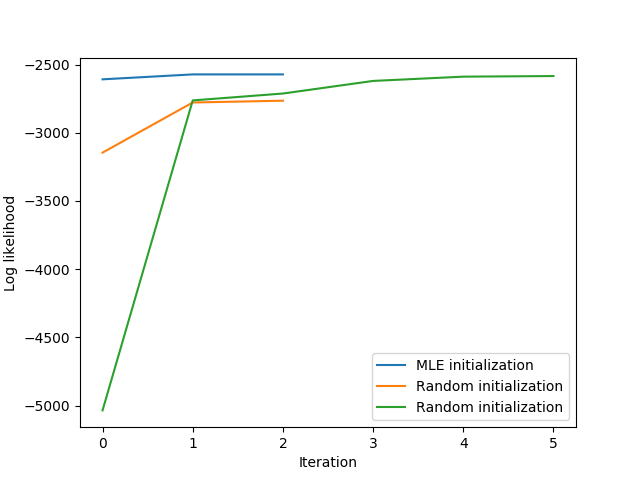
\includegraphics{starter/2aii.png}
				\caption{Log-likelihood of simple mixture of gaussians model for 3 different initializations}
				\label{fig:2aii}
			\end{figure}

  	\end{enumerate}
  \item Geography-aware Mixture Model
  	\begin{enumerate}[label=(\roman*)]
  		\item We first explicitly write out the entire log likelihood in terms of our parameters, where we now define $\theta = (\phi, \lambda, \mu_0, \mu_1, \Sigma_0, \Sigma_0)$. We have:
  		\begin{align*}
  			\ell\ell(\mathcal{D}\mid \theta) &= \left(\sum_{i=1}^N \sum_{j=1}^M \log \mathcal{N}(x_{ij} \mid \mu_{z_{ij}}, \Sigma_{z_{ij}})\right) \\
  			&+ \left(\sum_{i=1}^N \sum_{j=1}^M (1 - |z_{ij} - y_i|)\log \lambda + (|z_{ij} - y_i|)\log(1 - \lambda) \right) \\
  			&+ M\sum_{i=1}^N y_i \log \phi + (1-y_i)\log (1 -\phi)
  		\end{align*}
  		We can immediately note the similarity between this log-likelihood and the one from the previous model in Part A. In fact, we note that the estimates $\mu_0, \mu_1, \Sigma_0$ and $\Sigma_1$ will remain unchanged. We can also note that the estimat for $\phi$ is very similar to our estimate for $\pi$ previously, so we have:
  		$$
  			\phi = \frac{1}{N}\sum_{i=1}^N y_i
  		$$
  		Similary, we have the estimate for $\lambda$ as:
  		$$
  			\lambda = \frac{1}{NM} \sum_{i=1}^N \sum_{j=1}^M (1 - |z_{ij} - y_i|)
  		$$
  		After running the code with the given labeled data, we find the estimate to be:
  		\begin{align*}
				\phi_{MLE} &= 0.6 \\
				\lambda_{MLE} &= 0.93
  		\end{align*}
  		\item 1
  	\end{enumerate}
\end{enumerate}

\end{document}
